\chapter{Framework}\label{cap.framework}
This chapter serves as a way to introduce the tools that I have employed during the development of this project. All of them are \textbf{open-source}. The transparency provided by the open-source platforms is a major advantage because the software can be joined together and adapted to our specific application, which is mainly written in \textbf{Python} \footnote{\url{https://www.python.org/}}.

\section{JdeRobot}\label{jderobot}
\textbf{JdeRobot} \footnote{\url{http://jderobot.org}} is an open source middleware for robotics and computer vision. It has been designed to simplify the software development in these fields. It's mostly written in C++ language and it's structured like a collection of components (tools and drivers) that communicate to each other through \textbf{ICE interfaces} \footnote{\url{https://zeroc.com/products/ice}}. It is also compatible with \textbf{ROS} \footnote{\url{http://www.ros.org/}}, which allows us to use ROS nodes and JdeRobot components simultaneously. This flexibility makes it very useful for our application.
We're going to employ its \textit{cameraserver} driver to capture images from different video sources.

\subsection*{\textit{cameraserver}}\label{cameraserver}
According to JdeRobot documentation, this driver can serve both real cameras and video files. It interacts with other components thanks to the \textit{Camera} interface.

In order to use \textit{cameraserver}, we have to properly set its configuration file. These are the parameters that we must specify:
\begin{itemize}
    \item A network address where the server is going to be listening.
    \item Parameters related with the video stream: URI, frame rate, image size, format.
\end{itemize}

\section{Keras}\label{keras}
As stated by \textbf{Keras} documentation \cite{chollet2015keras}: "Keras is a high-level neural network library, written in Python and capable of running on top of either TensorFlow or Theano". TensorFlow and Theano are open-source libraries for numerical computation optimized for GPU and CPU that Keras treats as its "backends". This Currently, I'm running Keras on top of \textbf{Theano} \footnote{\url{http://deeplearning.net/software/theano/index.html}} optimized for CPU, but it's quite easy to switch from one backend to another.

We're going to analyze the main elements that make up a neural network built with Keras, starting with the \textit{model} object, its core component.

\subsection*{Models}\label{models}
Every neural network in Keras is defined as a \textit{model}. For those neural networks which can be built as a stack of \textit{layers} \ref{layers}, Keras provides the \textit{\textbf{Sequential model}} object. It is also possible to build more complex models with multiple outputs and shared layers using the Keras \textit{functional API}.

{\color{red}{SEQUENTIAL MODEL METHODS!!}}

\subsection*{Layers}\label{layers}
As it has been said before, the models are usually built as a stack of layers. These layers are added to the model using the \textit{.add()} method, inside of which the kind of layer is declared and its particular parameters are set. Several kinds of layers are available, but only the ones that have been used in this project are going to be described:
\begin{description}
	\item[Convolutional layer] This particular layer is the one that turns the neural network into a \textbf{convolutional neural network (CNN)}. They are formed by a fixed number of filters/kernels with a fixed size. These filters are convolved along the input image, generating each one a feature or activation map which will tell us whether the feature learned by that particular filter is present in the input image or not. Keras provides different kinds of convolutional layers depending on the input dimensions: \textit{Conv1D}, \textit{Conv2D} and \textit{Conv3D}. These are the main arguments required by Keras to define a convolutional layer:
	\begin{itemize}
		\item \textbf{\textit{filters}}: number of filters.
		\item \textbf{\textit{kernel\_size}}: width and height of the filters.
		\item \textbf{\textit{strides}}: how many pixels the filter must be shifted before applying the next convolution. Output size depends on this parameter. It defaults to 1.
		\item \textbf{\textit{padding}}: it can be \textit{valid} or \textit{same}. If \textit{valid} mode is set, no padding is applied, resulting in a reduced output. However, if \textit{same} mode is set, the input will be padded with zeros in order to produce an output that preserves the input size. It defaults to \textit{valid}
	\end{itemize}
\end{description}
\begin{description}
	\item[{Pooling layer}] It shifts a window of a certain size along the input (e.g. a feature map) applying an operation (mean or maximum) that will return a condensed version of it. Depending on the dimensions of the input and the operation applied, Keras provide several pooling layers: MaxPooling1D, MaxPooling2D, MaxPooling3D, AveragePooling1D... The main arguments required by Keras to define these layers are:
	\begin{itemize}
		\item \textbf{\textit{pool\_size}}: size of the window that is shifted along the input. It can also be interpreted as the factor by which the input is going to be downsampled.
		\item \textbf{\textit{strides}}: how many pixels the window must be shifted before applying the desired operation.
	\end{itemize}
\end{description}
\begin{description}
	\item[Dense layer] Fully-connected layers in Keras are defined as \textit{Dense layers}. In a \textbf{fully-connected layer}, every neuron is connected to every activation (output) of the previous one. The main argument of this layer is:
	\begin{itemize}
		\item \textbf{\textit{units}}: number of neurons.
	\end{itemize} 
\end{description}
\begin{description}
	\item[Activation layers] In Keras models, activations can be declared employing the \textit{.add()} method, or as an argument of the corresponding layer. Keras provides several \textbf{activation functions}, such as sigmoid, linear, ReLU and softmax. The only argument that must be provided to activation layers is the name of the desired activation function. These are the ones that have been used during the development of the project:
	\begin{itemize}
		\item \textbf{ReLU (Rectified Linear Unit)}: This activation function introduces non-linearity right after each convolutional layer, allowing the CNN to learn more complex features. It's defined as:
		\begin{equation}
		g(z)=\max(0,z)
		\end{equation}
		\item \textbf{Softmax} This activation function is very useful in the output layer of classification tasks. It takes a vector of real values $z$ and returns a new vector of real values in the range [0,1]. The $N$ lements of the output vector can be considered probabilities because the softmax function ensures that they sum up to 1. It is defined as follows:
		\begin{equation}
		\mathrm{softmax}(z)_i=\frac{\exp(z_i)}{\Sigma_{j}{\exp(z_j)}} \quad \mathrm{for} \ j=1, ...,N
		\end{equation}
	\end{itemize}
	This equations (Goodfellow et al., 2016 \cite{Goodfellow-et-al-2016}) are equivalent to the ones employed by Keras, defined by its backends Theano and Tensorflow.
\end{description}
\begin{description}
	\item[Flatten layer] It "flattens" the input. For instance, it converts the activation maps returned by the convolutional layers into a vector of neurons before being connected to a dense layer. It takes no arguments.
\end{description}
\begin{description}
	\item[Dropout layer] It's considered a regularization layer, because it's main purpose is to avoid over-fitting. Dropout (Srivastava et al., 2014 \cite{Srivastava-et-al-2014})it's a technique that randomly "switches-off" a fraction of hidden units during training (both forward and backward propagation). This layer, as other regularization layers (i.e. GaussianNoise layer), is only active during training. It's main argument is:
	\begin{itemize}
		\item \textbf{\textit{rate}}: fraction of units that must be dropped.
	\end{itemize}
\end{description}
\subsection*{Image Preprocessing}
\subsection*{Losses}
\subsection*{Metrics}
\subsection*{Optimizers}
\subsection*{Callbacks}
\subsection*{Utils}
Keras include a module for multiple supplementary tasks called \textbf{Utils}. The most important functionality for the project provided by this module is the \textbf{\textit{.HDF5Matrix()} method}. It reads the \textbf{HDF5} \footnote{\url{https://support.hdfgroup.org/HDF5/doc/H5.format.html}} datasets that are going to be used as inputs to the neural networks.

\section{Scikit-Learn}
\textbf{Scikit-Learn} \footnote{\url {http://scikit-learn.org/stable/index.html}} is a machine learning library that includes a wide variety of algorithms for clustering, regression and classification. It can be used during the whole machine learning process: preprocessing, training, model selection and evaluation.

We're going to employ Scikit-Learn functions to evaluate the neural networks that we have developed with Keras. Using a tool that is independent from Keras allows us to compare the results achieved by different neural network libraries (e.g. Keras and Caffe).

\section{Octave}
\textbf{GNU Octave} \footnote{\url{https://www.gnu.org/software/octave/}} is a scientific programming language compatible with Matlab. It provides powerful tools for plotting. We're going to use these tools to visualize the data collected with Scikit-Learn about the performance of our models. An example of a visualization using Octave can be seen in the figure \ref{figura:conf_mat}.
\begin{figure}
	\centering
	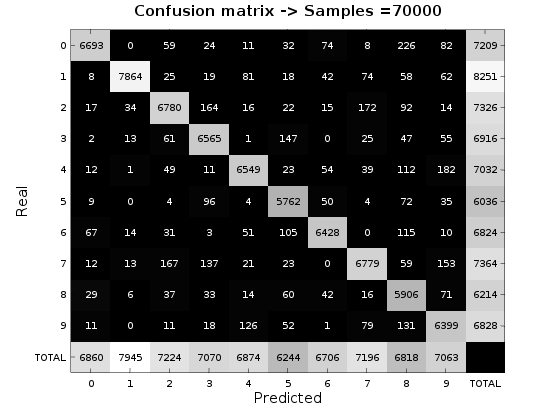
\includegraphics[width=12cm, keepaspectratio]{figures/conf_mat.png}
	\caption{Example of a confusion matrix visualization using Octave.}
	\label{figura:conf_mat}
\end{figure}